%!TEX root = ../../report.tex
\section{Collaborative Recommendations}
\label{sec:collaborative}
The main idea of this approach for recommendations, is to base the recommendations of items on similar users or similar items.\newline
This method of recommending is one of the most widely spread, as it is used both at Amazon, Netflix and similar high-value companies \citep{AmazonRecommendations}.\newline
In this section, the different implementation techniques of CF recommender systems will be described and a list of advantages and disadvantages will be given towards the end. We will distinguish between what is known as user-based and item-based recommendations \citep{IntroductionRecommenderSystems}.Before going into these descriptions, a short section for the common features will be explained\newline
For both types of recommendations the basic problem can be formulated like this: For any given user and non-rated item, try to estimate the rating the user will give for this item.\newline
The most common approach is therefore to define a user-item matrix as seen in the table below.


\begin{table}[H]
\begin{center}
\begin{tabular}{l c c c c c c r }
  & Item1 & Item2 & Item3 & Item4 & Item5 \\ 
 Alice & 5 & 3 & 4 & 4 & ? \\
 UserA & 3 & 1 & 2 & 3 & 3 \\
 UserB & 4 & 3 & 4 & 3 & 5 \\
 UserC & 3 & 3 & 1 & 5 & 4 \\
 UserD & 1 & 5 & 5 & 2 & 1
\end{tabular}
\caption{User-item matrix \(R\)}
\label{tableofratings} 
\end{center}
\end{table}



\subsection{User-user-based recommendations} % (fold)
\label{sub:user_user_based_recommendations}
The approach described here are recommending on the basis of what is known as peer-users (also called neighbors), which means users that have similar preferences as the user the system is trying to recommend items to. The idea is: For item \(n\), which a user called \(Alice\) have not yet rated, find peer-users that have rated item \(n\) and based on this, compute the rating for item \(n\) for \(Alice\). This means that the job of the RS is to: 1) find peer-users with similar taste to \(Alice\) and 2) take the rating for item \(n\) from the peer-users and based on this, predict the rating for item \(n\) for \(Alice\).\newline
To illustrate this, we return to the user-item matrix \(R\) in \ref{tableofratings}. Here \(Alice\) have not rated item 5 and the task of the recommender system is therefore to predict the rating for item 5, based on the ratings for this item from peer-users. Most commonly the peer-users are found by using the Pearson correlation coefficient\citep{IntroductionRecommenderSystems}, which calculates the similarity between users.

\subsubsection{Pearson correlation}
Before describing the mathematical formulations, we first need to establish the basic terms required for the calculations. As described in section \ref{sec:collaborative} a matrix of items and users are used. The users will in the following be denoted as \( U = {u_{1}, \ldots , u_{n}} \) , the items will be denoted as \( P = {p_{1}, \ldots , p_{n}} \) and \(R\) for the \({n \times m}\) matrix for ratings \(r_{i}, r_{j}\) for \(i \in 1 \ldots n, j \in 1 \ldots m\). The possible ratings a user can give is 1-5, where 5 being the the most-liked rating option. 
The similarity between two users \(a\) and \(b\), given the matrix \(R\) is defined as follows:\\

\[
	sim(a,b) = \frac{\sum_{p\in P} (r_{a,p} - \bar{r_{a}})(r_{b,p} - \bar{r_{b}})}{\sqrt{\sum_{p\in P} (r_{a,p} - \bar{r_{a}})^2} \sqrt{\sum_{p\in P} (r_{b,p} - \bar{r_{b}})^2}}
\]


Doing this for each of the users and \(Alice\) will produce the similarity between \(Alice\) and each of the other users. The RS will then take the users with the highest similarity and proceed. In this example the most similar users are \(userB\) and \(userC\). It should be noted, that the formula takes into account that users tends to interpret a rating scale differently. Meaning that, some users tend to give a lot of high ratings, whereas other never rates anything with a 5\citep[p. 15]{IntroductionRecommenderSystems}.\newline 
Now that we have found two users (\(B\) and \(C\)), that are similar to \(Alice\), we are able to proceed and predict the rating for \(Item5\), which \(Alice\) not yet have rated. According to \citet[p. 16]{IntroductionRecommenderSystems} one possible way of making the prediction is based on this formula, where $\bar{r_{a}}$ is the average of \(Alice's\) ratings,  :\newline

\[
	pred(a,p) = \bar{r_{a}} + \frac{\sum_{b\in N} sim(a,b) * (r_{b,p} - \bar{r_{b}})}{\sum_{b\in N} sim(a,b)}
\]
which produces the following: \newline

\[
	pred(a,p) = 4 + \frac{0,85*(3-2,4)+0,70*(5-3,8)}{0,85+0,70} = 4,87
\]
Based on these predictions, we are now able to fill out the user-item matrix for \(Alice\) and make a list of top recommendations. The list of recommendations is a product of both computed ratings, using the above method, and actual ratings from \(Alice\). \newline

The above presentation of a recommender systems is of course a very small example and in real world applications, the case of recommending is not as straight-forward as the method described here. The example just holds 5 users and 5 items, whereas real-world applications often contains tens of thousands or even millions of both items and users, as in the case with the Netflix Prize, which contained 480,000, 18,000 movie titles \citep{NetflixPrize}. As we will later present, a problem about data sparsity with rating of items, is also a very present and problematic issue for recommendation systems.\newline
This concludes the description of the user-user based recommendation technique and the second type of collaborative recommendations technique will be described next.
% subsection user_user_based_recommendations (end) 

\subsection{Item-based recommendations} % (fold)
\label{sub:item_based_recommendations}
Another technique of collaborative recommendations, called item-based, are in certain areas very similar to the user-based technique described above. The main idea of this approach is to calculate the similarity between items, instead of users, based on ratings for the items. If we want to compute the rating for \(Item5\) and we return to the matrix in \ref{tableofratings}, we can see that the all ratings given for \(Item5\), is close to all the ratings given for both \(Item1\) and \(Item4\). Because of this similarity, we can conclude the following: Since \(Alice\) gave a rating of 5 to \(Item1\) and gave a rating of 4 to \(Item4\), an item-based recommender system will compute the average of these similar items ratings and give \(Item5\) a rating between 4 and 5.

\subsubsection{Cosine similarity measure}
In the previous sections we looked at how \(Item5\) had similar ratings with \(Item1\) and \(Item4\). Because of a small dataset, it was possible to observe this similarity without any kind of calculations. It is rarely the case that this is possible in real-world applications and one of the methods for calculating this similarity is to use the cosine similarity measure. \newline 
By making a vector for each of the items, based on their ratings, this method uses the angle between two vectors for finding their similarity. The formula for calculating this angle is found below:

\[
	sim(\vec{a}, \vec{b}) = \frac{\vec{a} \cdot \vec{b}}{|\vec{a}| * |\vec{b}| }
\]
\newline
The cosine similarity values goes from -1, trough 0 and to 1, where 1 indicates a strong similarity between the two compared items, just like the Pearson method, as indicated on the picture below:

\begin{figure}[H]
\centering
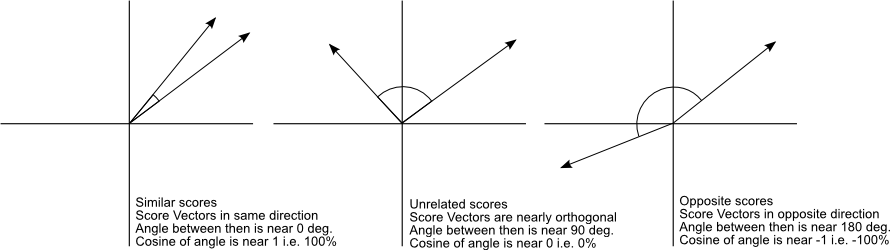
\includegraphics[width=90mm]{Pictures/cosinesimilarity.png}
\caption{source: http://pyevolve.sourceforge.net/wordpress/?p=2497}
\label{cosinesimilarity}
\end{figure}

Differently from the Pearson method, does this formula not take into account that users use a rating scale differently. To take this into account, the \textit{adjusted} cosine measure could be used:

\[
	sim(a,b) = \frac{\sum_{u \in U}(r_{u,a} - \bar{r_{u}})*(r_{u,b} - \bar{r_{u}})}{\sqrt{\sum_{u \in U}(r_{u,a} - \bar{r_{u}})^2}\sqrt{\sum_{u \in U} (r_{u,b} - \bar{r_{u}})^2}}
\]
After the similarity between the items have been calculated, the recommender system can predict a rating for \(Alice's\) \(Item5\), based on the ratings for the items similar to \(Item5\). This prediction is done, using the formula below:

\[
	pred(u,p) = \frac{\sum_{i\in ratedItems(u)} sim(i,p) * r_{u,i}}{\sum_{i \in ratedItems(a)} sim(i,p)}
\]

According to \citet{AmazonRecommendations} this is the specific method implemented in the webshop of Amazon.com. The reason for choosing this, over the user-user based approach, is for reasons of scalability. The user-based algoritm does not scale well, when the user and item space becomes large. 

\subsection{Advantages and disadvantages}
Collaborative recommender systems is one of the most researched techniques of the different types of recommendation systems and because of this, many different types of collaborative recommendations exists \citep{IntroductionRecommenderSystems}. For all these different types, it is possible to outline some common advantages and disadvantages, which will be done in this section.\newline

One of the big advantages, compared to Content-based recommendations (which will be explained in section \ref{sec:content}), are the fact that collaborative filtering works independently of the items it recommends. The only thing needed to produce recommendations are ratings, even if the items are dissimilar to those seen in the past \citep[p. 18]{TowardsTheNextGenerationOfRs}. This does, however, also mean that the system are very depended upon ratings, which means that the system are very vulnerable, if no ratings are given. Another advantage is the possibility of adding new items. Compared to Content-based, new items can be added to the inventory without having to analyze the content of the item. But even though the process of adding new items are an easy and quick one, in order for the item to be recommended, it still relies on ratings.\newline 
Like with Content-based recommender method, the collaborative method do also have some disadvantages described here as: New user problem and data sparsity.\newline

\textbf{New user} problem, in common named Cold start problem, are related to new users entering the system. This could be the case, if a recommender system were to recommend a movie to a user, which the system does not have previous history of and the user haven't rated any movies. This is a general problem for both the Collaborative and Content based approach. \newline

\textbf{Data Sparsity} is a problem describing the lack of ratings within the system. Many recommendation systems suffer from this, since users tend not to rate items, and very often the available ratings are very small compared to the total number of ratings \citep[p. 19]{TowardsTheNextGenerationOfRs}. 

\newpage